\begin{center}
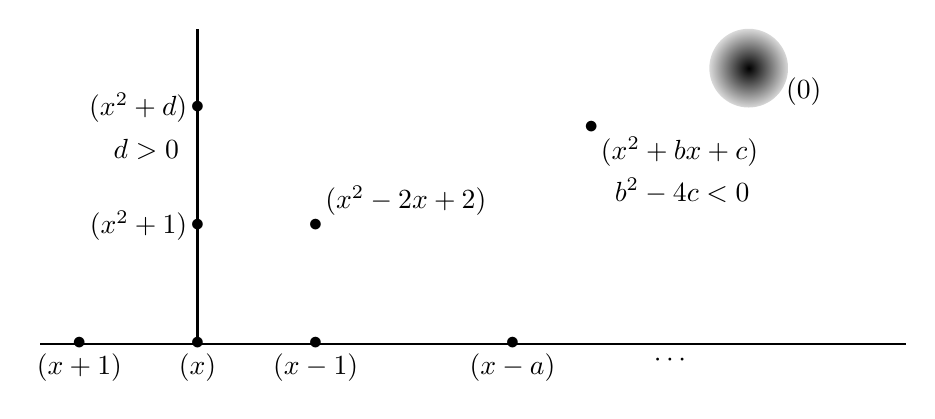
\begin{tikzpicture}

\draw[thick] (-1,0)
    -- (-0.5,0) node {$\bullet$} node[below] {$(x+1)$}
    -- (1,0) node {$\bullet$} node[below] {$(x)$}
    -- (2.5,0) node {$\bullet$} node[below] {$(x-1)$}
    -- (5,0) node {$\bullet$} node[below] {$(x-a)$}
    -- (7,0) node[below] {$\cdots$}
    -- (10,0);
\draw[thick] (1,0)
    -- (1,1.5) node {$\bullet$} node[left] {$(x^2 + 1)$}
    -- (1,3) node {$\bullet$} node[left] {$(x^2 + d)$} node[left, yshift=-15, xshift=-3] {$d > 0$}
    -- (1,4);
\draw (2.5,1.5) node {$\bullet$} node[above right] {$(x^2 - 2x + 2)$};
\draw (6,2.75) node {$\bullet$} node[below right] {$(x^2 + bx + c)$} node[below right,yshift=-15,xshift=5] {$b^2 - 4c < 0$};

\shade[inner color=black, outer color=gray!30] (8,3.5) circle (0.5);
\draw (8.7,3.2) node {$(0)$};
\end{tikzpicture}
\end{center}